% \definecolor{mauLa}{HTML}{EFE2BA} 
% \definecolor{mauL1}{HTML}{C5CBE3} 
% \definecolor{mauL2}{HTML}{D79922} 
% \definecolor{mauL3}{HTML}{4056A1} 
% \definecolor{mauL4}{HTML}{F13C20} 

% \section{Algorithm Visualization}

% \subsection{Huffman Algorithm Steps}

% \begin{enumerate}[label=\textbf{\Alph*.}]
%     \item \textbf{Count the Symbols' Frequencies}
%     \begin{itemize}
%         \item Read the input and count the frequency of each symbol in the data.
%         \item The frequencies indicate how often each symbol appears in the input data.
%         \begin{table}[h!]
%         \centering
%         \begin{tabular}{|c|c|}
%         \hline
%         \rowcolor{gray!30}
%         Symbol & Frequency \\
%         \hline
%         a & 5 \\
%         b & 9 \\
%         c & 12 \\
%         d & 13 \\
%         e & 16 \\
%         f & 45 \\
%         \hline
%         \end{tabular}
%         \caption{All symbols and their Frequencies}
%         \end{table}
%     \end{itemize}

%     \item \textbf{Build a Min-Heap (Priority Queue)}
%     \begin{itemize}
%         \item Insert each symbol as a node into a Min-heap based on its frequency.
%         \item The highest priority is given to the symbols with the least frequency.

%         \begin{figure}[H]
%         \centering
%         \begin{tikzpicture}
%           [level distance=1.8cm,
%            level 1/.style={sibling distance=4cm},
%            level 2/.style={sibling distance=3cm}]
%           \node[circle, draw=mauLa, fill=mauLa!60] {a | 5}
%             child {node[circle, draw=mauLa, fill=mauLa!60] {b | 9}
%               child {node[circle, draw=mauLa , fill=mauLa!60] {d | 13}}
%               child {node[circle, draw=mauLa , fill=mauLa!60] {e | 16}}
%             }
%             child {node[circle, draw=mauLa, fill=mauLa!60] {c | 12}
%               child {node[circle, draw=mauLa , fill=mauLa!60] {f | 45}}
%             };
%         \end{tikzpicture}
%         \caption{Step 1: Build a Min-Heap (Priority Queue)}
%         \end{figure}
%     \end{itemize}

%     \item \textbf{Construct the Huffman Tree}
%     \begin{itemize}
%         \item Extract the two nodes with the lowest frequency from the heap.
%         \item Merge them into a new node, with the frequency of this node being the sum of the two frequencies.
%         \item Insert the newly created node back into the heap.
%         \item Repeat this step until there is only one node left in the heap. This node will be the root of the Huffman tree.
%     \end{itemize}

%     \item \textbf{Assign Binary Codes to Symbols}
%     \begin{itemize}
%         \item Use a traversal algorithm to traverse the Huffman tree from the root and assign binary codes to each symbol following these rules:
%         \begin{itemize}
%             \item When passing the left edge, add '0' to the binary string.
%             \item When passing the right edge, add '1' to the binary string.
%             \item When reaching a leaf, use the binary string to assign the symbol in that node.
%         \end{itemize}
%         \item All symbols are leaf nodes, ensuring that no symbol is in the path of another symbol from the root, making the binary code a prefix code.
%     \end{itemize}

%     \item \textbf{Encode the Data}
%     \begin{itemize}
%         \item Replace all symbols with the Huffman codes that have been assigned to them.
%     \end{itemize}

%     \item \textbf{Decode the Data}
%     \begin{itemize}
%         \item Use the Huffman tree to find the symbols assigned by the codes in the encoded file.
%         \item Start from the root and read the encoded file bit by bit:
%         \begin{itemize}
%             \item When encountering bit '1', go to the right edge.
%             \item When encountering bit '0', go to the left edge.
%             \item When reaching a leaf, print the symbol in that node.
%         \end{itemize}
%         \item Return to the root and repeat until the end of the file is reached.
%     \end{itemize}
% \end{enumerate}

% \subsection{Huffman Tree Construction}
% The following figures illustrate the construction of the Huffman tree:

% \begin{figure}[H]
%     \centering
%     \begin{minipage}{0.5\textwidth}
%         \centering
%         \begin{tikzpicture}
%           [level distance=1.8cm,
%            level 1/.style={sibling distance=4cm},
%            level 2/.style={sibling distance=2cm}]
%           \node[circle, draw=mauLa , fill=mauLa!60] {a | 5}
%             child {node[circle, draw=mauLa , fill=mauLa!60] {b | 9}
%               child {node[circle, draw=mauLa , fill=mauLa!60] {d | 13}}
%               child {node[circle, draw=mauLa , fill=mauLa!60] {e | 16}}
%             }
%             child {node[circle, draw=mauLa , fill=mauLa!60] {c | 12}
%               child {node[circle, draw=mauLa , fill=mauLa!60] {f | 45}}
%             };
%         \end{tikzpicture}
%     \end{minipage}
%     \hfill
%     \begin{minipage}{0.25\textwidth}
%         \centering
%         \begin{tabular}{|c|c|}
%             \hline
%             \rowcolor{gray!30}
%             Symbol & Frequency \\
%             \hline
%             a & 5 \\
%             b & 9 \\
%             c & 12 \\
%             d & 13 \\
%             e & 16 \\
%             f & 45 \\
%             \hline
%         \end{tabular}
%     \end{minipage}
%     \caption{Step 1: Build a Min-Heap (Priority Queue)}
% \end{figure}

% \begin{figure}[H]
%     \centering
%     \begin{minipage}{0.5\textwidth}
%         \centering
%         \begin{tikzpicture}
%           [level distance=1.8cm,
%            level 1/.style={sibling distance=4cm}]
%           \node[circle, draw=mauL1, fill=mauL1!60] {T1 | 14}
%             child {node[circle, draw=mauLa , fill=mauLa!60] {a | 5}}
%             child {node[circle, draw=mauLa , fill=mauLa!60] {b | 9}};
%         \end{tikzpicture}
%     \end{minipage}
%     \hfill
%     \begin{minipage}{0.25\textwidth}
%         \centering
%         \begin{tabular}{|c|c|}
%             \hline
%             \rowcolor{gray!30}
%             Symbol & Frequency \\
%             \hline
%             c & 12 \\
%             T1 & 14 \\
%             d & 13 \\
%             e & 16 \\
%             f & 45 \\
%             \hline
%         \end{tabular}
%     \end{minipage}
%     \caption{Step 2: Initial Tree}
% \end{figure}

% \begin{figure}[H]
%     \centering
%     \begin{minipage}{0.5\textwidth}
%         \centering
%         \begin{tikzpicture}
%           [level distance=1.8cm,
%            level 1/.style={sibling distance=4cm},
%            level 2/.style={sibling distance=3cm}]
%           \node[circle, draw=mauL2, fill=mauL2!60] {T2 | 26}
%             child {node[circle, draw=mauLa , fill=mauLa!60] {c | 12}}
%             child {node[circle, draw=mauL1, fill=mauL1!60] {T1 | 14}
%               child {node[circle, draw=mauLa , fill=mauLa!60] {a | 5}}
%               child {node[circle, draw=mauLa , fill=mauLa!60] {b | 9}}
%             };
%         \end{tikzpicture}
%     \end{minipage}
%     \hfill
%     \begin{minipage}{0.25\textwidth}
%         \centering
%         \begin{tabular}{|c|c|}
%             \hline
%             \rowcolor{gray!30}
%             Symbol & Frequency \\
%             \hline
%             d & 13 \\
%             e & 16 \\
%             T2 & 26 \\
%             f & 45 \\
%             \hline
%         \end{tabular}
%     \end{minipage}
%     \caption{Step 3: After First Merge}
% \end{figure}

% \begin{figure}[H]
%     \centering
%     \begin{minipage}{0.5\textwidth}
%         \centering
%         \begin{tikzpicture}
%           [level distance=1.8cm,
%            level 1/.style={sibling distance=4cm}]
%           \node[circle, draw=mauL1, fill=mauL1!60] {T3 | 29}
%             child {node[circle, draw=mauLa , fill=mauLa!60] {d | 13}}
%             child {node[circle, draw=mauLa , fill=mauLa!60] {e | 16}};
%         \end{tikzpicture}
%     \end{minipage}
%     \hfill
%     \begin{minipage}{0.25\textwidth}
%         \centering
%         \begin{tabular}{|c|c|}
%             \hline
%             \rowcolor{gray!30}
%             Symbol & Frequency \\
%             \hline
%             T2 & 26 \\
%             T3 & 29 \\
%             f & 45 \\
%             \hline
%         \end{tabular}
%     \end{minipage}
%     \caption{Step 4: After Second Merge}
% \end{figure}

% \begin{figure}[H]
%     \centering
%     \begin{minipage}{0.5\textwidth}
%         \centering
%         \begin{tikzpicture}
%           [level distance=1.8cm,
%            level 1/.style={sibling distance=6cm},
%            level 2/.style={sibling distance=4cm},
%            level 3/.style={sibling distance=3cm}]
%           \node[circle, draw=mauL3, fill=mauL3!60] {T4 | 55}
%             child {node[circle, draw=mauL2, fill=mauL2!60] {T2 | 26}
%               child {node[circle, draw=mauLa , fill=mauLa!60] {c | 12}}
%               child {node[circle, draw=mauL1, fill=mauL1!60] {T1 | 14}
%                 child {node[circle, draw=mauLa , fill=mauLa!60] {a | 5}}
%                 child {node[circle, draw=mauLa , fill=mauLa!60] {b | 9}}
%                 }
%             }
%             child {node[circle, draw=mauL1, fill=mauL1!60] {T3 | 29}
%               child {node[circle, draw=mauLa , fill=mauLa!60] {d | 13}}
%               child {node[circle, draw=mauLa , fill=mauLa!60] {e | 16}}
%             };
%         \end{tikzpicture}
%     \end{minipage}
%     \hfill
%     \begin{minipage}{0.25\textwidth}
%         \centering
%         \begin{tabular}{|c|c|}
%             \hline
%             \rowcolor{gray!30}
%             Symbol & Frequency \\
%             \hline
%             f & 45 \\
%             T4 & 55 \\
%             \hline
%         \end{tabular}
%     \end{minipage}
%     \caption{Step 5: After Third Merge}
% \end{figure}

% \begin{figure}[H]
%     \centering
%     \begin{minipage}{0.5\textwidth}
%         \centering
%         \begin{tikzpicture}
%           [level distance=1.8cm,
%            level 1/.style={sibling distance=6cm},
%            level 2/.style={sibling distance=6cm},
%            level 3/.style={sibling distance=4cm},
%            level 4/.style={sibling distance=4cm}]
%            \node[circle, draw=mauL4, fill=mauL4!60]{T5 | 100}
%             child {node[circle, draw=mauLa , fill=mauLa!60] {f | 45}}
%             child {node[circle, draw=mauL3, fill=mauL3!60] {T4 | 55}
%                 child {node[circle, draw=mauL2, fill=mauL2!60] {T2 | 26}
%                   child {node[circle, draw=mauLa , fill=mauLa!60] {c | 12}}
%                   child {node[circle, draw=mauL1, fill=mauL1!60] {T1 | 14}
%                     child {node[circle, draw=mauLa , fill=mauLa!60] {a | 5}}
%                     child {node[circle, draw=mauLa , fill=mauLa!60] {b | 9}}
%                     }
%                 }
%                 child {node[circle, draw=mauL1, fill=mauL1!60] {T3 | 29}
%                   child {node[circle, draw=mauLa , fill=mauLa!60] {d | 13}}
%                   child {node[circle, draw=mauLa , fill=mauLa!60] {e | 16}}
%                 }
%             };
%         \end{tikzpicture}
%     \end{minipage}
%     \hfill
%     \begin{minipage}{0.25\textwidth}
%         \centering
%         \begin{tabular}{|c|c|}
%             \hline
%             \rowcolor{gray!30}
%             Symbol & Frequency \\
%             \hline
%             T5 & 100 \\
%             \hline
%         \end{tabular}
%     \end{minipage}
%     \caption{Step 6: After Fourth Merge}
% \end{figure}

% \subsection{Huffman Codes}
% Now, to generate code from this tree, we’ll traverse it from the root and assign 0 to left child and 1 to the right child. Once we encounter the leaf node, we may print this code.


% \begin{figure}[H]
%     \centering
%     \begin{minipage}{0.5\textwidth}
%         \centering
% \begin{tikzpicture}  
%   [level distance=1.8cm,  
%    level 1/.style={sibling distance=6cm},  
%    level 2/.style={sibling distance=6cm},  
%    level 3/.style={sibling distance=4cm},  
%    level 4/.style={sibling distance=4cm}]  
%    \node[circle, draw=mauL4, fill=mauL4!60]{T5 | 100}  
%     child {node[circle, draw=mauLa , fill=mauLa!60] {f | 45}  
%       edge from parent node[midway, left=0.2cm, fill=white, inner sep=1pt] {0} % Trọng số cạnh trái  
%     }  
%     child {node[circle, draw=mauL3, fill=mauL3!60] {T4 | 55}  
%         child {node[circle, draw=mauL2, fill=mauL2!60] {T2 | 26}  
%           child {node[circle, draw=mauLa , fill=mauLa!60] {c | 12}  
%             edge from parent node[midway, left=0.2cm, fill=white, inner sep=1pt] {0}  
%           }  
%           child {node[circle, draw=mauL1, fill=mauL1!60] {T1 | 14}  
%             child {node[circle, draw=mauLa , fill=mauLa!60] {a | 5}  
%               edge from parent node[midway, left=0.2cm, fill=white, inner sep=1pt] {0}  
%             }  
%             child {node[circle, draw=mauLa , fill=mauLa!60] {b | 9}  
%               edge from parent node[midway, right=0.2cm, fill=white, inner sep=1pt] {1}  
%             }  
%             edge from parent node[midway, right=0.2cm, fill=white, inner sep=1pt] {1}  
%           }  
%           edge from parent node[midway, left=0.2cm, fill=white, inner sep=1pt] {0}  
%         }  
%         child {node[circle, draw=mauL1, fill=mauL1!60] {T3 | 29}  
%           child {node[circle, draw=mauLa , fill=mauLa!60] {d | 13}  
%             edge from parent node[midway, left=0.2cm, fill=white, inner sep=1pt] {0}  
%           }  
%           child {node[circle, draw=mauLa , fill=mauLa!60] {e | 16}  
%             edge from parent node[midway, right=0.2cm, fill=white, inner sep=1pt] {1}  
%           }  
%           edge from parent node[midway, right=0.2cm, fill=white, inner sep=1pt] {1}  
%         }  
%         edge from parent node[midway, right=0.2cm, fill=white, inner sep=1pt] {1}  
%     };  
% \end{tikzpicture}      
% \end{minipage}
%     \hfill
%     \begin{minipage}{0.25\textwidth}
%         \centering
%         \begin{tabular}{|c|c|c|}
%         \hline
%         \rowcolor{gray!30}
%         Symbol & Code & ASCII \\
%         \hline
%         a & 1010 & 1100001 \\
%         b & 1011 & 1100010 \\
%         c & 100 & 1100011 \\
%         d & 110 & 1100100 \\
%         e & 111 & 1100101 \\
%         f & 0 & 1100110 \\
%         \hline
%         \end{tabular}
%     \end{minipage}
%     \caption{All of Symbols and their codes}
% \end{figure}

\definecolor{mauLa}{HTML}{EFE2BA}   
\definecolor{mauL1}{HTML}{C5CBE3}   
\definecolor{mauL2}{HTML}{D79922}   
\definecolor{mauL3}{HTML}{4056A1}   
\definecolor{mauL4}{HTML}{F13C20}   

\section{Algorithm Visualization}  

\subsection{Huffman Algorithm Steps}  

\begin{enumerate}[label=\textbf{\Alph*.}]  
    \item \textbf{Count the Symbols' Frequencies}  
    \begin{itemize}  
        \item Read the input and count the frequency of each symbol in the data.  
        \item The frequencies indicate how often each symbol appears in the input data.  
        \begin{table}[h!]  
        \centering  
        \begin{tabular}{|c|c|}  
        \hline  
        \rowcolor{gray!30}  
        Symbol & Frequency \\
        \hline  
        H & 1 \\
        u & 1 \\
        m & 1 \\
        a & 1 \\
        n & 1 \\
        f & 2 \\
        \hline  
        \end{tabular}  
        \caption{All symbols and their frequencies in "Huffman"}  
        \end{table}  
    \end{itemize}  

    \item \textbf{Build a Min-Heap (Priority Queue)}  
    \begin{itemize}  
        \item Insert each symbol as a node into a Min-heap based on its frequency.  
        \item The highest priority is given to the symbols with the least frequency.  

        \begin{figure}[H]  
        \centering  
        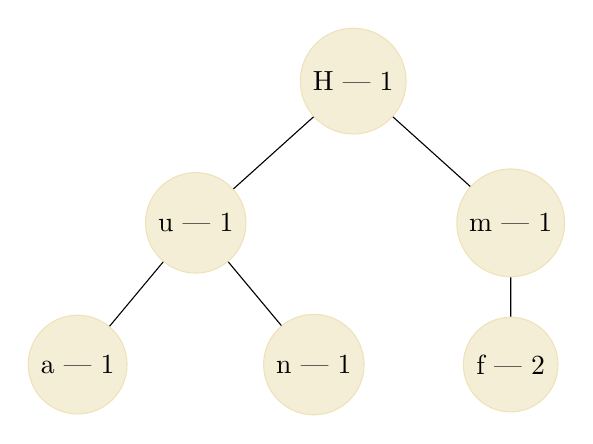
\begin{tikzpicture}  
          [level distance=1.8cm,  
           level 1/.style={sibling distance=4cm},  
           level 2/.style={sibling distance=3cm}]  
          \node[circle, draw=mauLa, fill=mauLa!60] {H | 1}  
            child {node[circle, draw=mauLa, fill=mauLa!60] {u | 1}  
              child {node[circle, draw=mauLa , fill=mauLa!60] {a | 1}}  
              child {node[circle, draw=mauLa , fill=mauLa!60] {n | 1}}  
            }  
            child {node[circle, draw=mauLa, fill=mauLa!60] {m | 1}  
              child {node[circle, draw=mauLa , fill=mauLa!60] {f | 2}}  
            };  
        \end{tikzpicture}  
        \caption{Step 1: Build a Min-Heap (Priority Queue)}  
        \end{figure}  
    \end{itemize}  

    \item \textbf{Construct the Huffman Tree}  
    \begin{itemize}  
        \item Extract the two nodes with the lowest frequency from the heap.  
        \item Merge them into a new node, with the frequency of this node being the sum of the two frequencies.  
        \item Insert the newly created node back into the heap.  
        \item Repeat this step until there is only one node left in the heap. This node will be the root of the Huffman tree.  
    \end{itemize}  

    \item \textbf{Assign Binary Codes to Symbols}  
    \begin{itemize}  
        \item Use a traversal algorithm to traverse the Huffman tree from the root and assign binary codes to each symbol following these rules:  
        \begin{itemize}  
            \item When passing the left edge, add '0' to the binary string.  
            \item When passing the right edge, add '1' to the binary string.  
            \item When reaching a leaf, use the binary string to assign the symbol in that node.  
        \end{itemize}  
        \item All symbols are leaf nodes, ensuring that no symbol is in the path of another symbol from the root, making the binary code a prefix code.  
        
        \begin{table}[h!]  
        \centering  
        \begin{tabular}{|c|c|}  
        \hline  
        \rowcolor{gray!30}  
        Symbol & Huffman Code \\
        \hline  
        H & 000 \\
        u & 001 \\
        f & 11 \\
        m & 010 \\
        a & 011 \\
        n & 10 \\
        \hline  
        \end{tabular}  
        \caption{Huffman codes for "Huffman"}  
        \end{table}  
    \end{itemize}  

    \item \textbf{Encode the Data}  
    \begin{itemize}  
        \item Replace all symbols with the Huffman codes that have been assigned to them.  
        \item For the string "Huffman", the encoded bit sequence is:  
        \begin{center}  
        \begin{tabular}{|c|c|}  
        \hline  
        \rowcolor{gray!30}
        Symbol & Code \\
        \hline  
        H & 000 \\
        u & 001 \\
        f & 11 \\
        f & 11 \\
        m & 010 \\
        a & 011 \\
        n & 10 \\
        \hline  
        \end{tabular}  
        \end{center}  
        
        \begin{center}  
        Complete encoded string: 000 001 11 11 010 011 10  
        \end{center}  
    \end{itemize}  

    \item \textbf{Decode the Data}  
    \begin{itemize}  
        \item Use the Huffman tree to find the symbols assigned by the codes in the encoded file.  
        \item Start from the root and read the encoded file bit by bit:  
        \begin{itemize}  
            \item When encountering bit '1', go to the right edge.  
            \item When encountering bit '0', go to the left edge.  
            \item When reaching a leaf, print the symbol in that node.  
        \end{itemize}  
        \item Return to the root and repeat until the end of the file is reached.  
        \item Decoding process:  
        \begin{center}  
        \begin{tabular}{|c|c|c|}  
        \hline 
        \rowcolor{gray!30}
        Code & Symbol & Progress \\
        \hline  
        000 & H & H \\
        001 & u & Hu \\
        11 & f & Huf \\
        11 & f & Huff \\
        010 & m & Huffm \\
        011 & a & Huffma \\
        10 & n & Huffman \\
        \hline  
        \end{tabular}  
        \end{center}  
    \end{itemize}  
\end{enumerate}  

\subsection{Huffman Tree Construction for "Huffman"}  
The following figures illustrate key steps in the construction of the Huffman tree for the string "Huffman":  

\begin{figure}[H]  
    \centering  
    \begin{minipage}{0.5\textwidth}  
        \centering  
        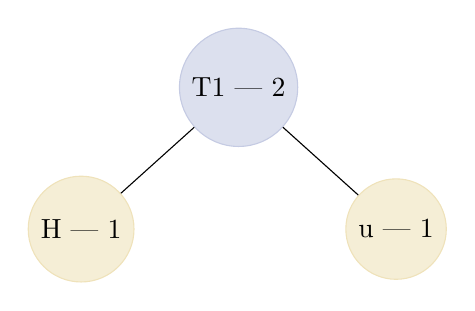
\begin{tikzpicture}  
          [level distance=1.8cm,  
           level 1/.style={sibling distance=4cm}]  
          \node[circle, draw=mauL1, fill=mauL1!60] {T1 | 2}  
            child {node[circle, draw=mauLa , fill=mauLa!60] {H | 1}}  
            child {node[circle, draw=mauLa , fill=mauLa!60] {u | 1}};  
        \end{tikzpicture}  
    \end{minipage}  
    \hfill  
    \begin{minipage}{0.25\textwidth}  
        \centering  
        \begin{tabular}{|c|c|}  
            \hline  
            \rowcolor{gray!30}  
            Symbol & Frequency \\
            \hline  
            m & 1 \\
            a & 1 \\
            n & 1 \\
            T1 & 2 \\
            f & 2 \\
            \hline  
        \end{tabular}  
    \end{minipage}  
    \caption{Step 2: First Merge - H and u}  
\end{figure}  

\begin{figure}[H]  
    \centering  
    \begin{minipage}{0.5\textwidth}  
        \centering  
        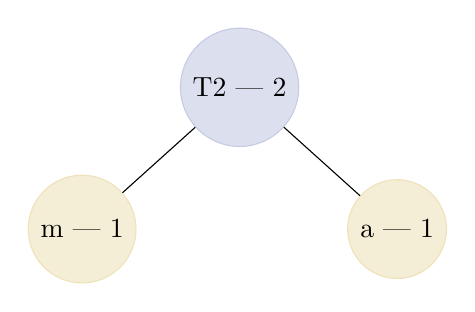
\begin{tikzpicture}  
          [level distance=1.8cm,  
           level 1/.style={sibling distance=4cm}]  
          \node[circle, draw=mauL1, fill=mauL1!60] {T2 | 2}  
            child {node[circle, draw=mauLa , fill=mauLa!60] {m | 1}}  
            child {node[circle, draw=mauLa , fill=mauLa!60] {a | 1}};  
        \end{tikzpicture}  
    \end{minipage}  
    \hfill  
    \begin{minipage}{0.25\textwidth}  
        \centering  
        \begin{tabular}{|c|c|}  
            \hline  
            \rowcolor{gray!30}  
            Symbol & Frequency \\
            \hline  
            n & 1 \\
            T1 & 2 \\
            T2 & 2 \\
            f & 2 \\
            \hline  
        \end{tabular}  
    \end{minipage}  
    \caption{Step 3: Second Merge - m and a}  
\end{figure}  

\begin{figure}[H]  
    \centering  
    \begin{minipage}{0.5\textwidth}  
        \centering  
        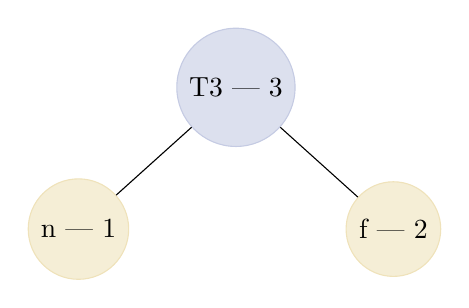
\begin{tikzpicture}  
          [level distance=1.8cm,  
           level 1/.style={sibling distance=4cm}]  
          \node[circle, draw=mauL1, fill=mauL1!60] {T3 | 3}  
            child {node[circle, draw=mauLa , fill=mauLa!60] {n | 1}}  
            child {node[circle, draw=mauLa , fill=mauLa!60] {f | 2}};  
        \end{tikzpicture}  
    \end{minipage}  
    \hfill  
    \begin{minipage}{0.25\textwidth}  
        \centering  
        \begin{tabular}{|c|c|}  
            \hline  
            \rowcolor{gray!30}  
            Symbol & Frequency \\
            \hline  
            T1 & 2 \\
            T2 & 2 \\
            T3 & 3 \\
            \hline  
        \end{tabular}  
    \end{minipage}  
    \caption{Step 4: Third Merge - n and f}  
\end{figure}  

\begin{figure}[H]  
    \centering  
    \begin{minipage}{0.5\textwidth}  
        \centering  
        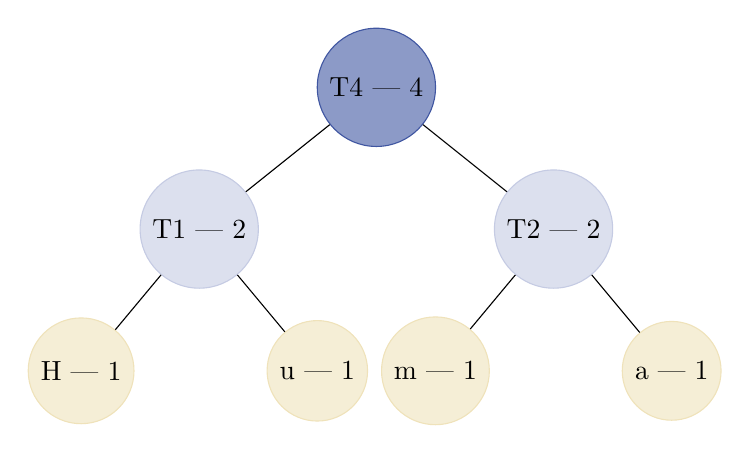
\begin{tikzpicture}  
          [level distance=1.8cm,  
           level 1/.style={sibling distance=4.5cm},  
           level 2/.style={sibling distance=3cm}]  
          \node[circle, draw=mauL3, fill=mauL3!60] {T4 | 4}  
            child {node[circle, draw=mauL1, fill=mauL1!60] {T1 | 2}  
              child {node[circle, draw=mauLa , fill=mauLa!60] {H | 1}}  
              child {node[circle, draw=mauLa , fill=mauLa!60] {u | 1}}  
            }  
            child {node[circle, draw=mauL1, fill=mauL1!60] {T2 | 2}  
              child {node[circle, draw=mauLa , fill=mauLa!60] {m | 1}}  
              child {node[circle, draw=mauLa , fill=mauLa!60] {a | 1}}  
            };  
        \end{tikzpicture}  
    \end{minipage}  
    \hfill  
    \begin{minipage}{0.25\textwidth}  
        \centering  
        \begin{tabular}{|c|c|}  
            \hline  
            \rowcolor{gray!30}  
            Symbol & Frequency \\
            \hline  
            T3 & 3 \\
            T4 & 4 \\
            \hline  
        \end{tabular}  
    \end{minipage}  
    \caption{Step 5: Fourth Merge - T1 and T2}  
\end{figure}  

\begin{figure}[H]  
    \centering  
    \begin{minipage}{0.5\textwidth}  
        \centering  
        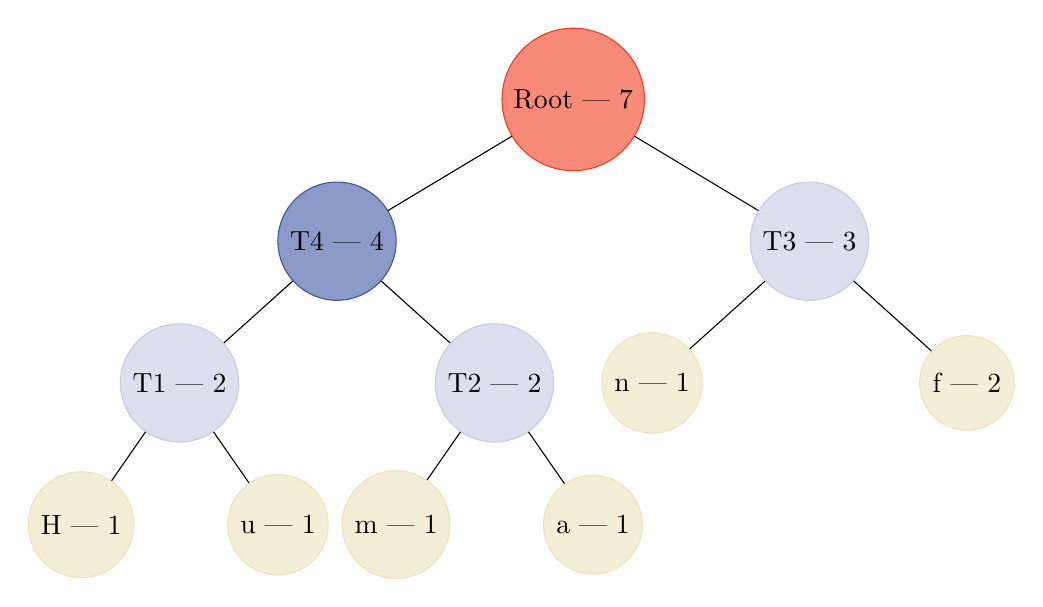
\begin{tikzpicture}  
          [level distance=1.8cm,  
           level 1/.style={sibling distance=6cm},  
           level 2/.style={sibling distance=4cm},  
           level 3/.style={sibling distance=2.5cm}]  
          \node[circle, draw=mauL4, fill=mauL4!60] {Root | 7}  
            child {node[circle, draw=mauL3, fill=mauL3!60] {T4 | 4}  
              child {node[circle, draw=mauL1 , fill=mauL1!60] {T1 | 2}  
                child {node[circle, draw=mauLa , fill=mauLa!60] {H | 1}}  
                child {node[circle, draw=mauLa , fill=mauLa!60] {u | 1}}  
                }  
              child {node[circle, draw=mauL1, fill=mauL1!60] {T2 | 2}  
                child {node[circle, draw=mauLa , fill=mauLa!60] {m | 1}}  
                child {node[circle, draw=mauLa , fill=mauLa!60] {a | 1}}  
                }  
            }  
            child {node[circle, draw=mauL1, fill=mauL1!60] {T3 | 3}  
              child {node[circle, draw=mauLa , fill=mauLa!60] {n | 1}}  
              child {node[circle, draw=mauLa , fill=mauLa!60] {f | 2}}  
            };  
        \end{tikzpicture}  
    \end{minipage}  
    \hfill  
    \begin{minipage}{0.25\textwidth}  
        \centering  
        \begin{tabular}{|c|c|}  
            \hline  
            \rowcolor{gray!30}  
            Symbol & Frequency \\
            \hline  
            Root & 7 \\
            \hline  
        \end{tabular}  
    \end{minipage}  
    \caption{Step 6: Final Merge - T3 and T4}  
\end{figure}  

\subsection{Huffman Codes}  
Following the tree construction, we traverse it from the root and assign 0 to left child and 1 to the right child. This gives us the Huffman codes shown below:  

\begin{center}
\begin{figure}[H]  
    \centering  
        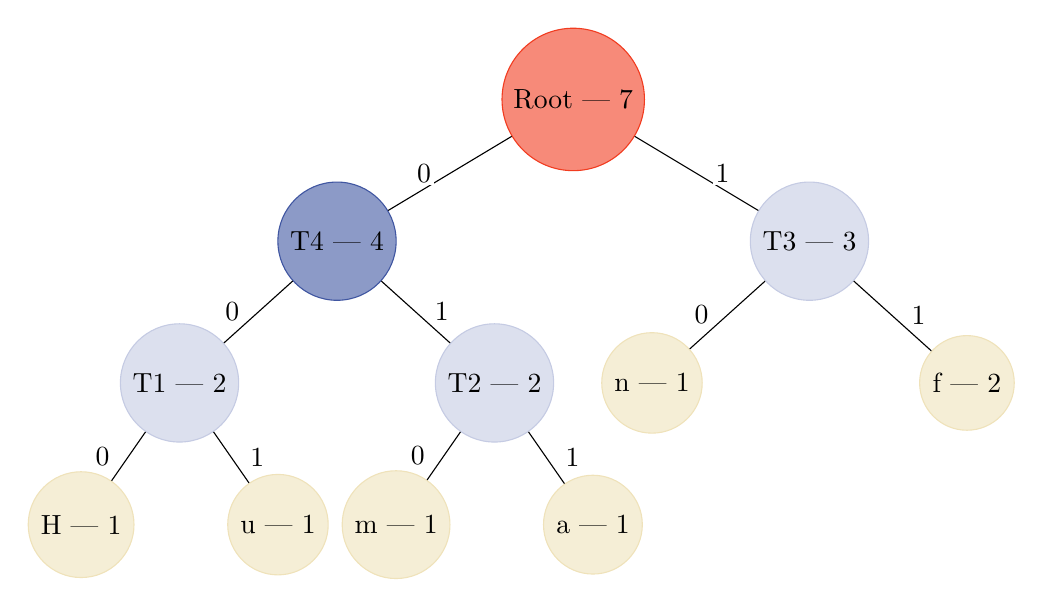
\begin{tikzpicture}  
          [level distance=1.8cm,  
           level 1/.style={sibling distance=6cm},  
           level 2/.style={sibling distance=4cm},  
           level 3/.style={sibling distance=2.5cm}]  
           \node[circle, draw=mauL4, fill=mauL4!60]{Root | 7}  
            child {node[circle, draw=mauL3, fill=mauL3!60] {T4 | 4}  
              child {node[circle, draw=mauL1 , fill=mauL1!60] {T1 | 2}  
                child {node[circle, draw=mauLa , fill=mauLa!60] {H | 1}  
                  edge from parent node[midway, left=0.2cm, fill=white, inner sep=1pt] {0}  
                }  
                child {node[circle, draw=mauLa , fill=mauLa!60] {u | 1}  
                  edge from parent node[midway, right=0.2cm, fill=white, inner sep=1pt] {1}  
                }  
                edge from parent node[midway, left=0.2cm, fill=white, inner sep=1pt] {0}  
              }  
              child {node[circle, draw=mauL1, fill=mauL1!60] {T2 | 2}  
                child {node[circle, draw=mauLa , fill=mauLa!60] {m | 1}  
                  edge from parent node[midway, left=0.2cm, fill=white, inner sep=1pt] {0}  
                }  
                child {node[circle, draw=mauLa , fill=mauLa!60] {a | 1}  
                  edge from parent node[midway, right=0.2cm, fill=white, inner sep=1pt] {1}  
                }  
                edge from parent node[midway, right=0.2cm, fill=white, inner sep=1pt] {1}  
              }  
              edge from parent node[midway, left=0.2cm, fill=white, inner sep=1pt] {0}  
            }  
            child {node[circle, draw=mauL1, fill=mauL1!60] {T3 | 3}  
              child {node[circle, draw=mauLa , fill=mauLa!60] {n | 1}  
                edge from parent node[midway, left=0.2cm, fill=white, inner sep=1pt] {0}  
              }  
              child {node[circle, draw=mauLa , fill=mauLa!60] {f | 2}  
                edge from parent node[midway, right=0.2cm, fill=white, inner sep=1pt] {1}  
              }  
              edge from parent node[midway, right=0.2cm, fill=white, inner sep=1pt] {1}  
            };  
        \end{tikzpicture}       
    \caption{Final Huffman tree with edge labels}  
\end{figure}  
\end{center}

\begin{figure}[H]  
    \centering    
        \centering  
        \begin{tabular}{|c|c|c|}  
        \hline  
        \rowcolor{gray!30}  
        Symbol & Huffman Code & ASCII (for comparison) \\
        \hline  
        H & 000 & 01001000 (8 bits) \\
        u & 001 & 01110101 (8 bits) \\
        f & 11 & 01100110 (8 bits) \\
        m & 010 & 01101101 (8 bits) \\
        a & 011 & 01100001 (8 bits) \\
        n & 10 & 01101110 (8 bits) \\
        \hline  
        \end{tabular}    
    \caption{All symbols and their Huffman codes for "Huffman"}  
\end{figure}  

\newpage
\subsection{Encoding Efficiency Analysis}  
\begin{itemize}  
    \item Original string "Huffman" (7 characters):  
    \begin{itemize}  
        \item ASCII encoding: $7 \times 8 = 56$ bits  
        \item Huffman encoding: $18$ bits (000 001 11 11 010 011 10)  
        \item Compression ratio: $(1 - 18/56) \times 100\% \approx 67.86\% $ savings. 
    \end{itemize}  
    \item The Huffman encoding provides significant compression by assigning shorter codes to more frequent symbols.  
    \item In this case, the character 'f' appears twice and receives the shortest code (11), while other characters receive longer codes.  
\end{itemize}  